\documentclass[submit]{harvardml}

\course{CS181-S24}
\assignment{Assignment \#2}
\duedate{11:59pm EST, Feb 23th, 2024}

\usepackage[OT1]{fontenc}
\usepackage[colorlinks,citecolor=blue,urlcolor=blue]{hyperref}
\usepackage[pdftex]{graphicx}
\usepackage{subfig}
\usepackage{fullpage}
\usepackage{amsmath}
\usepackage{amssymb}
\usepackage{framed}
\usepackage{color}
\usepackage{soul}
\usepackage{todonotes}
\usepackage{listings}
\usepackage{common}
\usepackage{enumitem}
\usepackage{bm}
\usepackage{bbm}
\newcommand{\B}{\text{B}}
\newcommand{\Beta}{\text{Beta}}

\usepackage[mmddyyyy,hhmmss]{datetime}

\definecolor{verbgray}{gray}{0.9}

\lstnewenvironment{csv}{%
  \lstset{backgroundcolor=\color{verbgray},
  frame=single,
  framerule=0pt,
  basicstyle=\ttfamily,
  columns=fullflexible}}{}




\begin{document}

\begin{center}
{\Large Homework 2: Classification and Bias-Variance Trade-offs}\\
\end{center}

\subsection*{Introduction}

This homework is about classification, bias-variance trade-offs, and
uncertainty quantification.

The datasets that we will be working with relate to astronomical
observations. The first dataset, found at \verb|data/planet-obs.csv|,
contains information on whether a planet was observed (as a binary
variable) at given points in time. This will be used in Problem 1. The
second dataset, available at \verb|data/hr.csv|, details different
kinds of stars and their measured magnitude and temperature. You will
work with this data in Problem 3.

As a general note, for classification problems we imagine that we have
the input matrix $\boldX \in \reals^{n \times d}$ (or perhaps they
have been mapped to some basis $\bm{\Phi}$, without loss of
generality) with outputs now ``one-hot encoded."  This means that if
there are~$K$ output classes, rather than representing the output
label $y$ as an integer~${1,2,\ldots,K}$, we represent $\boldy$ as a
``one-hot" vector of length~$K$. A ``one-hot" vector is defined as
having every component equal to 0 except for a single component which
has value equal to 1.  For example, if there are $K = 7$ classes and a
particular data point belongs to class 3, then the target vector for
this data point would be~$\boldy = [0,0,1,0,0,0,0]$.  We will define
$C_1$ to be the one-hot vector for the 1st class, $C_2$ for the 2nd
class, etc.  Thus, in the previous example $\boldy = C_3$. If there
are $K$ total classes, then the set of possible labels is $\{C_1
\ldots C_K \} = \{C_k\}_{k=1}^K$.  Throughout the assignment we will
assume that each label $\boldy \in \{C_k\}_{k=1}^K$ unless otherwise
specified. The most common exception is the case of binary
classification ($K = 2$), in which case labels are the typical
integers $y \in \{0, 1\}$.

\subsection*{Resources and Submission Instructions}

We encourage you to read CS181 Textbook's Chapter 3 for more
information on linear classification, gradient descent, and
classification in the discriminative setting. Read Chapter 2.8 for
more information on the trade-offs between bias and variance.

In problems 1 and 3, you may use \texttt{numpy} or \texttt{scipy}, but
not \texttt{scipy.optimize} or \texttt{sklearn}. Example code is given
in the provided notebook.

Please type your solutions after the corresponding problems using this
\LaTeX\ template, and start each problem on a new page.

Please submit the \textbf{writeup PDF to the Gradescope assignment
  `HW2'}. Remember to assign pages for each question.  Please submit
your \textbf{\LaTeX\ file and code files to the Gradescope assignment
  `HW2 - Supplemental'}. \textbf{You must include your plots in your
  writeup PDF. } The supplemental files will only be checked in
special cases, e.g. honor code issues, etc.


%%%%%%%%%%%%%%%%%%%%%%%%%%%%%%%%%%%%%%%%%%%%%
% Problem 1
%%%%%%%%%%%%%%%%%%%%%%%%%%%%%%%%%%%%%%%%%%%%%

\begin{problem}[Exploring Bias-Variance and Uncertainty]
In this problem, we will explore the bias and variance of a few
different model classes when it comes to logistic regression and
investigate two sources of predictive uncertainty in a synthetic
(made-up) scenario.

We are using a powerful telescope in the northern hemisphere to gather
measurements of some planet of interest. At certain times however, our
telescope is unable to detect the planet due to its positioning around
its star.  The data in \verb|data/planet-obs.csv| records the
observation time in the ``Time" column and whether the planet was
detected in the ``Observed" column (with the value 1 representing that
it was observed).  These observations were taken over a dark, clear
week, which is representative of the region.  Since telescope time is
expensive, we would like to build a model to help us schedule and find
times when we are likely to detect the planet.

\begin{enumerate}
\item Split the data into 10 mini-datasets of size $N = 30$ (i.e. dataset 1 consists of the first 30 observations, dataset 2 consists of the next 30, etc. This has already been done for you). Consider the three bases $\boldsymbol\phi_1(t) = [1, t]$, $\boldsymbol\phi_2(t) = [1,
  t, t^2]$, and $\boldsymbol\phi_3(t) = [1, t, t^2, t^3, t^4, t^5]$. For each of these bases, fit a logistic regression model using sigmoid($\boldw^\top \boldsymbol\phi(t)$) to each dataset by using gradient descent to
  minimize the negative log-likelihood.  This means you will be
  running gradient descent 10 times for each basis, once for each
  dataset.
  
  Use the given starting values of $\boldw$ and a learning rate of $\eta=0.001$, take 10,000 update
  steps for each gradient descent run, and make sure to average the
  gradient over the data points at each step. These parameters,
  while not perfect, will ensure your code runs reasonably quickly. 

\item After consulting with a domain expert, we find that the probability of observing the planet is periodic as the planet revolves around its star---we are more likely to observe the planet when it is in front of its star than when it is behind it. In fact, the expert determines that observation follows the generating process $y \sim \text{Bern}(f(t))$, where $f(t) = 0.4 \times \cos(1.1t + 1) + 0.5$ for $t \in [0, 6]$ and $y \in \{0,1\}$. Note that we, the modelers, do not usually see the true data distribution. Knowledge of the true $f(t)$ is only exposed in this problem to allow for verification of the true bias.

Use the given code to plot the true process versus your learned models. Include your plots in your solution PDF.

\textbf{In no more than 5 sentences}, explain how bias and variance reflected in the 3 types of curves on the graphs.  How do the fits of the individual and mean prediction functions change?  Keeping in mind that none of the model classes match the true generating process exactly, discuss the extent to which each of the bases approximates the true process.

\end{enumerate}
\end{problem}

\newpage
\begin{framed}
\noindent\textbf{Problem 1} (cont.)\\
\begin{enumerate}
\setcounter{enumi}{2}

\item If we were to increase the size of each dataset drawn from $N = 30$ to a larger number, how would the bias and variance change for each basis? Why might this be the case? You may experiment with generating your own data that follows the true process and plotting the results, but this is \textbf{not} necessary. \textbf{Your response should not be longer than 5 sentences}.

\item Consider the test point $t = 0.1$. Using your models trained on basis $\boldsymbol\phi_3$, report the predicted probability of observation of the \textit{first} model (the model trained on the first 30 data points). How can we interpret this probability as a measure of uncertainty? Then, compute the variance of the classification probability over your 10 models at the same point $t = 0.1$. How does this measurement capture another source of uncertainty, and how does this differ from the uncertainty represented by the classification probability? Repeat this process (reporting the first model's classification probability and the variance over the 10 models) for the point $t = 3.2$.

  Compare the uncertainties and their sources at times $t=0.1$ and $t=3.2$.

\item We now need to make some decisions about when to request time on
  the telescope.  The justifications of your decisions will be sent to
  your funding agency, which will determine whether you will be
  allocated funds to use the telescope for your project.
  \begin{itemize}
  \item To identify the ideal time, which model(s) would you use and why?
  \item What time would you request, and why?
  \item Your funding agency suggests using a different telescope in a
    humid area near the equator. Can you still use your model to
    determine when the planet is likely to be visible?  Why? Are there
    adaptations that may be necessary?
  \item You seek out a team that has used the alternative telescope
    for observing this planet, and they provide you their observation
    file \verb|data/planet-obs-alternate.csv|.
    Compare the observations from your telescope to theirs.  What
    seems to be happening?  What might be an appropriate model for
    this? Your funding agency asks you to refit your models on these
    new data.  Do you think this is a reasonable ask, and if so, how
    will it help you make better decisions about when to request
    viewing time?  If not, why do you think the additional modeling
    will not help? You do \emph{not} need to do any modeling for this
    question!
  \item The team who shared the data tells you that the effect you're
    seeing is due to the weather around the telescope.  Weather
    forecasts for the area are usually accurate a few days in
    advance. Does that affect your strategy for requesting time?  If
    so, how?  If not, why not?
  \end{itemize}
  In these questions, we are looking for your reasoning; there may be
  more than one valid answer.

\end{enumerate}
\end{framed}

\newpage
\textbf{1.} I'm not entirely sure what the submittable portion of this problem is, because it is simplying saying to set up the way the model will be run,
so to avoid not submitting anything, I decided to submit my code in this section, which passed the tests that the question talks about. 
For this part of the problem, I changed the Code in Jupyter Notebook to the following. For Basis2 and Basis3 I wrote: \\
\begin{center}
  \includegraphics{basis_code.png}
\end{center}

Then, for the fit and predict functions, I wrote the following code: 
\begin{center}
  \includegraphics{fit_and_predict.png}
\end{center}

With these functions, I was able to make all three bases pass the test. \\\\

\textbf{2.} The plots I got are as given: 
\begin{center}
  \includegraphics[width=0.3\textwidth]{basis1.png} \includegraphics[width=0.3\textwidth]{basis2.png} \includegraphics[width=0.3\textwidth]{basis3.png}
\end{center}

From looking at these plots, it is apparent the relationship between variance and bias. In the first basis, which is the simplest, there is a high 
level of bias, as can be seen through the distance between the mean of the learned model and the ground truth of the dataset. Of the three graphs, the first basis has the most 
bias, but it also has a very low variance, because the line does not fit the data well. That means that outlying points will do comparitively little to sway the mean. This trend is 
continued with bases 2 and 3, with the trend being that as the complexity increases, the bias decreases, with the model fitting the data better, but also the curve gets 
increasingly more susceptible to variation from new points. The third basis has the best approximation of the true data in terms of bias, but also is prone to overfitting 
as seen in the irregular behaviors of the graph. \\\\

\textbf{3.} If we increased the size of each dataset to a larger number, that would lead to a decrease in bias across 
all three bases. This is because this increased N would allow each model more information to train on and would lead to a 
more informed approximation, which will have a lower bias than with less data points. The more data points there are though the 
more potential there is for variance. As data continues to be collected, that data picks up more on variability within what is being measured,
so the models are likely to have a higher variance. \\\\

\textbf{4.} I found that at the test point $t = 0.1$, Model 1, which is the first 30 data points, gives a predicted probability of $0.3482$, which 
can be interpreted by saying that the first model is .3482 certain that the planet is visible at that time. This means that because this value is closer to 0 
than it is to 1 that this model is relatively more certain that the planet is not visible at this time than that it is visible. Then I calulcated the variance of the answers 
that all ten models gave, and found that the variance between all ten models was 0.0049, indicating that there is not much variation at all between individual models. 
This also helps to quantify the uncertainty because it is clear to see that all ten of the models are very similar to each other, so all the models roughly agree that 
the probability is closer to 0 than 1, which make the assertion that the planet is not usually seen at time t = 1 even more certain. Then, when done again for t = 3.2, I found that
for model 1, the predicted probability at 3.2 was 0.6074, which again means that for model 1, there is a roughly 60\% chance that the planet can be seen at time 3.2, which means it 
is more likely to be present than not, but does not have a certainty or guarantee to be seen. When calculating the variance over the 10 model at time 3.2 I got Variance = 0.0056, which once again shows that all ten models agree 
pretty closely and increases the certainty of model 1's findings.  \\\\

\textbf{5.} To identify the ideal time, I would use the second model; the one based off of 
basis 2. That is because that model is in a nice sweet spot of not being overfit and having a reasonably small bias 
and also a reasonably small variance. Of the three bases, it is the most stable and accurate, so it is the best to use for 
analyzing the information. I would then request the time to be between time 4 and time 5, since those are times when the planet was 
very frequently spotted through the telescope, while also having a minimal mean squared error across that interval. If this project were to be moved 
to a more humid climate, the model found above will most likely not be applicable. These models are specific to a cloudless environment where 
there is no interference from weather, and in a different climate that is unlikely to also be the case, so different data must be collected to account 
for weather patterns and cloud patterns in the new area. Looking at the data provided in planet-obs-alternate, it appears that the alternate location has a very different 
graph for planet observation. The initial location has a much more sinusoidal nature to the curve of planet visibility, but it appears that the alternate dataset has much more consistent
visibility with no clear sinusoidal function to model it. Refiting the models to match this data makes sense because of the difference in distribution between the locations. This being
a result of the weather in the area makes sense and it does effect your request for time, because you want to make sure you avoid a time when there is no probability of seeing the planet just due 
to clouds being in the way. It would also be helpful in this case to prove that the clouds being there does not have a spurious connection to the planet being visible which is skewing the data, 
but it is still best to request time according to the weather patterns. 

%%%%%%%%%%%%%%%%%%%%%%%%%%%%%%%%%%%%%%%%%%%%%
% Problem 2
%%%%%%%%%%%%%%%%%%%%%%%%%%%%%%%%%%%%%%%%%%%%%

\begin{problem}[Maximum likelihood in classification, 15pts]

  Consider now a generative $K$-class model.  We adopt class prior
  $p(\boldy = C_k; \bpi) = \pi_k$ for all $k \in \{1, \ldots, K\}$
(where $\pi_k$ is a parameter of the prior).
Let  $p(\boldx|\boldy=C_k)$ denote
the class-conditional density of features $\boldx$ (in this
case for class $C_k$). Consider the data set $D = \{(\boldx_i,
\boldy_i)\}_{i=1}^n$ where as above $\boldy_i \in \{C_k\}_{k=1}^K$ is
encoded as a one-hot target vector and the data are independent.

\begin{enumerate}
  \item Write out the log-likelihood of the data set, $\ln p(D ; \bpi)$.

  \item Since the prior forms a distribution, it has the constraint that
    $\sum_k\pi_k - 1 = 0$.  Using the hint on
Lagrange multipliers below, give the
    expression for the maximum-likelihood estimator for the prior
    class-membership probabilities, i.e.
    $\hat \pi_k.$
    Make sure to write out the intermediary equation you need
    to solve to obtain this estimator. Briefly state why your final answer is intuitive.
\end{enumerate}

    For the remaining questions, let the
    class-conditional probabilities be Gaussian distributions with
the same covariance matrix
    $$p(\boldx | \boldy = C_k) = \mathcal{N}(\boldx |  \bmu_k, \bSigma), \text{\ for\ }k \in \{1,\ldots, K\}$$
    and different means $\bmu_k$ for each class.

    \begin{enumerate}
  \item[3.] Derive the gradient of the log-likelihood with respect to vector $\bmu_k$.
    Write the expression in matrix form as a function of the variables defined
    throughout this exercise. Simplify as much as possible for full credit.
  \item[4.] Derive the maximum-likelihood estimator $\hat{\mu}_k$ for vector $\bmu_k$. Briefly state why your final answer is intuitive.
  \item[5.] Derive the gradient for the log-likelihood with respect to the
    covariance matrix $\bSigma$ (i.e., looking
to find an MLE for the covariance).
Since you are differentiating with respect to a
    \emph{matrix}, the resulting expression should be a matrix!
%
  \item[6.] Derive the maximum likelihood estimator $\hat{\Sigma}$ of the covariance matrix.
\end{enumerate}

\paragraph{Hint: Lagrange Multipliers.} Lagrange Multipliers are a method for
optimizing a function $f$ with respect to an
equality constraint, i.e.
\[\min_{\boldx} f(\boldx)\ \text{s.t.}\ g(\boldx) = 0.\]

This can be turned into an unconstrained problem by introducing a
Lagrange multiplier $\lambda$ and constructing the Lagrangian function,
\[L(\boldx, \lambda) =  f(\boldx) + \lambda g(\boldx).\]

It can be shown that it is a necessary condition that the optimum
is a critical point of this new function. We can find this point by solving two equations:

\[\dfrac{\partial L(\boldx, \lambda)}{\partial  \boldx} = 0  \ \ \text{and}\  \  \dfrac{\partial L(\boldx, \lambda)}{\partial \lambda} = 0 \]


\paragraph{Cookbook formulas.} Here are some formulas you might want to consider
using to compute difficult gradients. You can use them  in the homework
without proof. If you are looking to hone your matrix calculus skills, try to
find different ways to prove these formulas yourself (will not be part of the
evaluation of this homework). In general, you can use any formula from the matrix cookbook,
as long as you cite it. We opt for the following common notation:
$\boldX^{-\top} := (\boldX^{\top})^{-1}$
\begin{align*}
  & \dfrac{\partial \bolda^\top \boldX^{-1} \boldb}{\partial \boldX} = - \boldX^{-\top} \bolda \boldb^\top \boldX^{-\top} \\
  & \dfrac{\partial \ln | \det (\boldX) |}{\partial \boldX} = \boldX^{-\top}
 \end{align*}
 \end{problem}

 \newpage 
 \textbf{1.} Since we want to say something about every data point $y_i$, we can make $n_k$ be equal to the amount of times in ${1,2, ... K}$ where $y_i = C_k$. 
 To find the log-likelihood of $P(D | \pi)$, we first must calculate the likelihood. Which is $\Pi_{i=1}^n [P(x_i, y_i) | \pi] = \Pi_{i=1}^n P(x_i | y_i, \pi) P(y_i | \pi)$.
 That gives us the probability of the data given $\pi$. But more important than $\pi$ is the idea that only when $y_i = C_k$ will the value by non-zero, just by definition of one-hot encoding.
 This means we can rewrite the probability as $\Pi_{i=1}^n [P(x_i | y_i = C_k)\pi_k]$. \\
 Then the next step is to take this equation and take the log of it, then using log rules: 
 \begin{center}
  $\ln[\Pi_{i=1}^n [P(x_i | y_i = C_k)\pi_k]] = \sum_{i=1}^{n} \ln(P(x_i|y_i = C_k)\pi_k) = \sum_{i=1}^{n} [\ln(P(x_i|y_i = C_k) + \ln(\pi_k))]$
 \end{center}
 Now from this we can complete the calculation using an indicator function, so that we only include values where $y_i = C_k$. We can define this as $\mathbb{I}(y_i = C_k)$ where $\mathbb{I}$ is 1 where $y_i = C_k$ and 0 otherwise.
 Then we can make two sums, one over all data points and the other which is to sum over all the non-zero data points, or points where $y_i \in n_k$With that defined we can now write it out fully as: 
 \begin{center}
    $\ln(P(D | \pi)) = \sum_{k=1}^{K} \sum_{i=1}^{n} \mathbb{I}(y_i = C_k)(\ln(P(x_i | y_i = C_k)) + ln(\pi_k))$
 \end{center}

 \textbf{2.} Using the hint given in the problem, we want to optimize the log likelihood, but use the constraint $\sum_{k} \pi_k - 1 = 0$. Then also using the hint, we know we can set this up as: 
 \begin{center}
    $L(\pi, \lambda) = \ln(P(D | \pi)) + \lambda(\sum_{k}\pi_k - 1)$ Then as per Part 1 $= \sum_{k=1}^{K} \sum_{i=1}^{n} \mathbb{I}(y_i = C_k)(\ln(P(x_i | y_i = C_k)) + ln(\pi_k)) + \lambda(\sum_{k}\pi_k - 1)$
 \end{center}
 Now, we want to solve for both $\dfrac{\partial L(\pi, \lambda)}{\partial \pi} = 0$ and $\dfrac{\partial L(\pi, \lambda)}{\partial \lambda} = 0$. Focusing on the first one with respect to pi, we can see that
 in order to solve this equation, we can think about it in terms of the sum from 1 to K of $\pi_k$, and so we can sum over all the data points to get that $\sum_{i=1}^{n}\dfrac{y_i}{\pi_k} + \lambda = 0$. Rearranging for $\pi_k$, 
 we get that $\pi_k = - \dfrac{\sum_{i=1}^{n} y_i}{\lambda}$ \\
 Next, we can solve for $\dfrac{\partial L(\pi, \lambda)}{\partial \lambda}$. This is simpler, because the first probability that we found in Part 1 above does not include any lambda terms, so we only need to take into account
 $\lambda(\sum_{k=1}^{K} \pi_k - 1)$. Then since this equation has lambda on the outside, the derivative is simply $\sum_{k=1}^{K} \pi_k - 1$. This leaves us with the equation $\sum_{k=1}^{K} \pi_k - 1 = 0$, then we can substitute
 the $\pi_k$ found above and get $\sum_{k=1}^{K} - \dfrac{\sum_{i=1}^{n} y_i}{\lambda} - 1 = 0$. Then, since we defined $n_k$ to be the number of values such that $y_i = C_k$, and those are the only nonzero additions, we know that 
 $\sum_{k=1}^{K} \sum_{i=1}^{n} y_i = \sum_{i=1}^{n} y_i = n_k$ just by nature of definition. This leaves us with the expression $\dfrac{n_k}{\lambda} = -1$, so $\lambda = -n_k$. Then using this, we can go back to the equation for $\pi_k$
 and we find that $\pi_k = \dfrac{n_k}{n}$. \\
 This makes intuitve sense because we want to maximize the size of $n_k$, so it makes sense to have the maximum parameter be the true proportion of those points in order to have the best representation. \\\\

 \textbf{3.} Again, in part one we found: $\ln(P(D | \pi)) = \sum_{k=1}^{K} \sum_{i=1}^{n} y_{ik}(\ln(P(x_i | y_i = C_k)) + ln(\pi_k))$, and now we can rewrite this given the class-conditioned probability as $\sum_{k=1}^{K} \sum_{i=1}^{n} y_{ik}(\ln(N(x_i | \mu_k, \Sigma))) + ln(\pi_k)$, 
 Now we want to take the gradient of this with respect to $\mu_k$ and we get: 
 \begin{center}
  $\dfrac{\partial}{\partial \mu_k} (\ln(P(D | \pi))) = \dfrac{\partial}{\partial \mu_k} [\sum_{k=1}^{K} \sum_{i=1}^{n} y_{ik}(\ln(N(x_i | \mu_k, \Sigma)))]$ \\
  $= \dfrac{\partial}{\partial \mu_k}[\sum_{k=1}^{K} \sum_{i=1}^{n} y_{ik} \ln(\dfrac{1}{\sqrt{2\pi\Sigma}} \exp(-\dfrac{(x_i - \mu_k)^T \Sigma^{-1} (x_i - \mu_k)}{2}))]$ \\
  $= \dfrac{\partial}{\partial \mu_k}[\sum_{i=1}^{n}-y_{ik}(\dfrac{(x_i - \mu_k)^T \Sigma^{-1} (x_i - \mu_k)}{2})]$.
 \end{center}
 Then we can use the Matrix Cookbook provided in the question to see that this is all equal to: 
 \begin{center}
    $\sum_{i=1}^{n} -y_{ik} \Sigma^{-1} (\mu_k - x_i) = \sum_{i=1}^{n} (\mathbb{I}(y_i = C_k))(-\Sigma^{-1} (\mu_k - x_i))$
 \end{center}

 \textbf{4.} For the maximum likelihood, we can take the equation we solved for in part 3 and just set it equal to 0: $\sum_{i=1}^{n} -y_{ik} \Sigma^{-1} (\mu_k - x_i)$, then we can 
 distribute the $y_{ik}$ since it is impacted by the sum and keep the $\Sigma^{-1}$ outside of the sum which leaves us with $\Sigma^{-1} \sum_{i=1}^{n}(-y_{ik}\mu_k + x_i y_{ik}) = \Sigma^{-1} [\mu_k\sum_{i=1}^{n}(-y_{ik}) + \sum_{i=1}^{n} x_i y_{ik}] = 0$.
 Then, since we want to solve for $\mu_k$, we don't care about $\Sigma^{-1}$ because it has no relevance to $\mu_k$, and we can rearrange to get that: 
 \begin{center}
    $\hat{\mu_k} = \dfrac{\sum_{i=1}^{n} x_i y_{ik}}{\sum_{i=1}^{n} y_{ik}}$.
 \end{center}
 Then, just as we did in the last part, we can rewrite this as the Indicator function to get that 
 \begin{center}
    $\hat{\mu_k} = \dfrac{\sum_{i=1}^{n} x_i \mathbb{I}(y_i = C_k)}{\sum_{i=1}^{n} \mathbb{I}(y_i = C_k)}$
 \end{center} 
 Once again this answer is intuitive because it shows that the maximum likelihood approximates the sum of all x values of a class
 divided by all the points in the class, effectively giving an average of that class, which is the maximum likelihood. \\\\

 \textbf{5.} This question wants $\dfrac{\partial}{\partial \Sigma} [\ln(P(d | \pi))]$. \\
 Once again, we can build off the work we've done so far in this problem to write this more concretely as: 
 \begin{center}
  $\dfrac{\partial}{\partial \Sigma} [\ln(P(d | \pi))] = \dfrac{\partial}{\partial \Sigma}[\sum_{k=1}^{K} \sum_{i=1}^{n} y_{ik}(\ln(N(x_i | \mu_k, \Sigma))) + ln(\pi_k)] = \dfrac{\partial}{\partial \Sigma}[\sum_{k=1}^{K} \sum_{i=1}^{n} y_{ik}(\ln(N(x_i | \mu_k, \Sigma)))]$ \\
  $= \sum_{k=1}^{K} \sum_{i=1}^{n} y_{ik} \dfrac{\partial}{\partial \Sigma} \ln(\dfrac{1}{\sqrt{2\pi\Sigma}}) + \ln(\exp(-\dfrac{(x_i - \mu_k)^T \Sigma^{-1} (x_i - \mu_k)}{2}))$ \\
  $= \sum_{k=1}^{K} \sum_{i=1}^{n} y_{ik} \dfrac{\partial}{\partial \Sigma} \left[\ln(\dfrac{1}{\sqrt{2\pi}}) + \ln(\Sigma^{-0.5})-\dfrac{(x_i - \mu_k)^T \Sigma^{-1} (x_i - \mu_k)}{2}\right]$
 \end{center}
 From there, we can once again use the cookbook formulas and simplify this as: 
 \begin{center}
  $\sum_{k=1}^{K} \sum_{i=1}^{n} y_{ik} \left(-\dfrac{1}{2} \Sigma^{-T} + \dfrac{\Sigma^{-T}(x_i - \mu_k)(x_i - \mu_k)^T \Sigma^{-T}}{2}\right)$
 \end{center}
 And we finish once again by putting it in terms of the indicator function to get 
 \begin{center}
  $\sum_{k=1}^{K} \sum_{i=1}^{n} \mathbb{I}(y_i = C_k) \left(-\dfrac{1}{2} \Sigma^{-T} + \dfrac{\Sigma^{-T}(x_i - \mu_k)(x_i - \mu_k)^T \Sigma^{-T}}{2}\right)$
 \end{center}

 \textbf{6.} Very similar to Problem 4, we can find the Maximum Likelihood just by setting our answer in part 5 equal to 0 and solving. First, we can pull the term 
 $\dfrac{1}{2}\Sigma^{-T}$ from the Sums because it does not depend on $k$ or $i$. As we pull it out though, we have to acknowledge that it will be multiplied by $n_k$, 
 or the number of times that $y_i = C_k$, so we can rewrite this as $-\dfrac{n}{2}\Sigma^{-T} + \sum_{k=1}^{K} \sum_{i=1}^{n} y_{ik} \left(\dfrac{\Sigma^{-T}(x_i - \mu_k)(x_i - \mu_k)^T \Sigma^{-T}}{2}\right)$, 
 then we can subtract that over to get $\sum_{k=1}^{K} \sum_{i=1}^{n} y_{ik} \left(\dfrac{\Sigma^{-T}(x_i - \mu_k)(x_i - \mu_k)^T \Sigma^{-T}}{2}\right) = \dfrac{n}{2} \Sigma^{-T}$. \\
 Now we can multiply $\Sigma^T$ on the left and right of both sides to eliminate the $\Sigma^{-T}$, which results in: 
 \begin{center}
  $\sum_{k=1}^{K} \sum_{i=1}^{n} y_{ik} \left(\dfrac{(x_i - \mu_k)(x_i - \mu_k)^T}{2}\right) = \dfrac{n}{2} \Sigma^{T}$, so we have
  $\Sigma^T = \sum_{k=1}^{K} \sum_{i=1}^{n} \mathbb{I}(y_i = C_k) \left(\dfrac{(x_i - \mu_k)(x_i - \mu_k)^T}{n}\right)$
 \end{center}

%%%%%%%%%%%%%%%%%%%%%%%%%%%%%%%%%%%%%%%%%%%%%
% Problem 3
%%%%%%%%%%%%%%%%%%%%%%%%%%%%%%%%%%%%%%%%%%%%%

\begin{problem}[Classifying Stars]
In this problem, you will code up three different classifiers to classify different types of stars. The file \verb|data/hr.csv| contains data on magnitude and temperature. The data can be plotted on these two axes:
\begin{center}
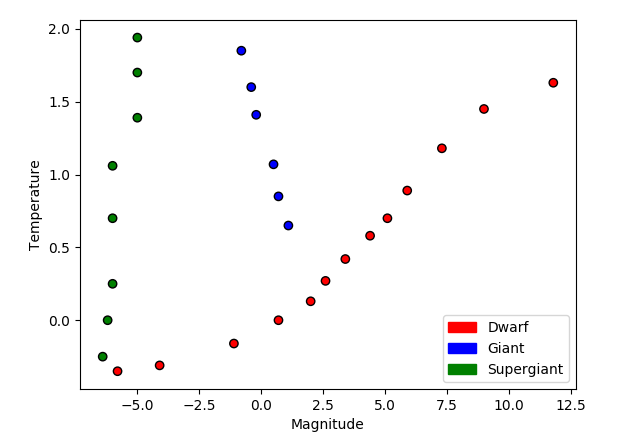
\includegraphics[width=.5\textwidth]{images/star.png}
\end{center}

Please implement the following classifiers in the \verb|SoftmaxRegression| and \verb|KNNClassifier| classes:

\begin{enumerate}[label=\alph*)]

\item \textbf{A generative classifier with Gaussian class-conditional
  densities with a \textit{shared covariance} matrix} across all classes. 
  Feel free to re-use your Problem 2 results.

\item \textbf{Another generative classifier with Gaussian class-conditional densities , but now 
with a \textit{separate covariance} matrix} learned for each class. (Note: 
The staff implementation can switch between the two Gaussian generative classifiers with just a
few lines of code.)

\item \textbf{A multi-class logistic regression classifier} using the softmax activation function. In your implementation of gradient descent, \textbf{make sure to include a bias term and use L2 regularization} with regularization parameter $\lambda = 0.001$. Limit the number of iterations of gradient descent to 200,000, and set the learning rate to be $\eta = 0.001$.

\item \textbf{Another multi-class logistic regression classifier} with feature map $\phi(\boldx) = [\ln (x_1 + 10), x_2^2]^\top$, where $x_1$ and $x_2$ represent the values for magnitude and temperature, respectively.

\item \textbf{A kNN classifier} in which you classify based on the $k = 1$ and $k = 5$ nearest neighbors and the following distance function: $$dist(star_1, star_2) = (mag_1 - mag_2)^2/9 + (temp_1 - temp_2)^2$$
where nearest neighbors are those with the smallest distances from a given point.

  Note 1: When there are more than two labels, no label may have the
  majority of neighbors.  Use the label that has the most votes among
  the neighbors as the choice of label. 

  Note 2: The grid of points for which you are making predictions
  should be interpreted as our test space.  Thus, it is not necessary
  to make a test point that happens to be on top of a training point
  ignore itself when selecting neighbors.

\end{enumerate}

After implementing the above classifiers, complete the following exercises:

\begin{enumerate}
    \item Plot the decision boundaries generated by each classifier for the dataset. Include them in your PDF. 
    Identify the similarities and differences among the classifiers. What explains the differences---in particular, which aspects or properties of each model dictate the shape of its decision boundary? 
    
    \item 
    
    Consider a star with Magnitude 3 and Temperature -2. To which class does each classifier assign this star? Report the classification probabilities of this star for each model. 
    
    Interpret how each model makes its classification decision. What are the pros and cons of each interpretation? What else should we, the modelers, be aware of when making predictions on a test point ``far" from our training data? \textbf{Your response should no be longer than 5 sentences.}
\end{enumerate}
\end{problem}

\newpage
\textbf{Solution:} \\
\textbf{1.} I was able to make the following decision boundaries: 

\begin{center}
  Gaussian with Shared Covariance: \\
  \includegraphics[width=0.4\textwidth]{gaussian_generative_shared_covariance.png} \\

  Gaussian with Separate Covariance: \\ 
  \includegraphics[width=0.4\textwidth]{gaussian_generative_separate_covariance.png} \\

  Logistic Regression Classifier: \\
  \includegraphics[width=0.4\textwidth]{softmax_regression_result.png} \\

  Logistics Regression with Basis \\
  \includegraphics[width=0.4\textwidth]{softmax_regression_with_feature_map.png} \\

  kNN with k = 1: \\
  \includegraphics[width=0.4\textwidth]{knn_k1.png} \\

  kNN with k = 5: \\
  \includegraphics[width=0.4\textwidth]{knn_k5.png} \\

\end{center}
  \textbf{1.} There are many similarities and differences among the models. For similarities, the most obvious is that 
  each model is trying to accomplish the same thing: successfully classify the data into Dwarf, Giant, or Supergiant. Because of this, 
  most of the graphs have similar trends, where even though the shape or size of regions may differ, the general classification of that region of space remains the same. 
  Despite these similarities, there are also many differences between the models. This is because each model has distinct assumptions that underly their decision boundaries. 
  For example, the Generative Gaussian model with shared covariance operates in a linear decision boundary because it assumes there is a Gaussian distribution, and the same is said for 
  a Gaussian Distribution with Separate Covariances, which operates with a quadratic assumption. The Softmax boundary looks very distinct from the other two categories because it features 
  non-linear boundaries by way of the feature transformations. Making the softmax reliant on a basis above the two dimensions it is graphed on leads to nonlinear graphing and a distinct boundary 
  between classifications which isn't seen in kNN or Gaussian. The kNN decision boundaries are shaped that way because they are much more reliant on the actual data. kNN boundaries are not constrained to a certain mapping or plane, 
  but are very specialized to the shape of the graph and as such don't have a uniform appearance per-say
  
  \textbf{2.} Here is what the point (3, -2) would be classified as in each graph: \\
  Graph A: Dwarf \\
  Graph B: Dwarf \\
  Graph C: Dwarf \\
  Graph D: Supergiant \\
  Graph E: Dwarf \\
  Graph F: Dwarf \\

  For a Gaussian model, it makes its classification decision based on which Gaussian Distribution that point falls under. The pros of a Gaussian Distribution is that it is probabilistic in nature 
  and so allows for some variance within the classifications, but a con is that the boundary can only be expressed in a linear or quadratic boundary which underrepresents a lot of boundaries.
  The Softmax regression calculates the probabilities according to the softmax function and chooses the class with the highest probability as the predicted class of the star. A pro of the softmax regression is that 
  it can model complex and nonlinear decision boundaries, but a con is that can overfit or create too much "noise" in the process with a complex basis. Laslty, kNN operates 
  by making decision boundaries according to the data points around a given area, the classification of a point will be the same as the majority of the k-nearest points to it. A pro of this method is that 
  it allows for complex boundaries which can conform to almost any shape, but a con of kNN is that it requires a lot of computation on larger data sets and can be time-ineffective for that reason. As a modeler, 
  it is important to be aware of the dangers of extrapolation; even if a model fits well within the range of the data given, it may not be generalizable. 

%%%%%%%%%%%%%%%%%%%%%%%%%%%%%%%%%%%%%%%%%%%%%
% Name and Calibration
%%%%%%%%%%%%%%%%%%%%%%%%%%%%%%%%%%%%%%%%%%%%%
\subsection*{Name}
\textbf{Dan Tracy}
\subsection*{Collaborators and Resources}
Whom did you work with, and did you use any resources beyond cs181-textbook and your notes?
I got assistance from Students Teresa Lu-Remeo and Christine Lee, but most of the work was done independently.

\end{document}
